\section{9649 JC2 Preliminary Examination Paper 1}

\begin{problem}
    The terms in the sequence $\bc{u_n}$ satisfy the recurrence relation \[u_n = \frac12 u_{n-1} + 3.\]

    \begin{enumerate}
        \item Find an expression for $u_n$ in terms of $n$ in the case that $u_0 = 1$.
        \item Describe the behaviour of the sequence as $n$ tends to infinity.
    \end{enumerate}
\end{problem}
\begin{solution}
    \begin{ppart}
        The complementary solution is \[u_n^{(c)} = C \bp{\frac12}^n.\] Let $k$ be a particular solution. Then $k =  \frac12 k + 3$, so $k = 6$. Thus, the general solution is \[u_n = u_{n}^{(c)} + k = C \bp{\frac12}^n + 6.\] Since $u_0 = 1$, we have that $C = -5$, so \[u_n = -\frac{5}{2^n} + 6.\]
    \end{ppart}
    \begin{ppart}
        $u_n$ is increasing and converges to 6.
    \end{ppart}
\end{solution}

\begin{problem}
    \begin{enumerate}
        \item Suppose $S_1$ and $S_2$ are the column spaces of matrices $\mat A_1$ and $\mat A_2$, where \[\mat A_1 = \begin{pmatrix}1 & -1 & a \\ 0 & 0 & b \\ 0 & 0 & c\end{pmatrix} \quad \tand \quad \mat A_2 = \begin{pmatrix}1 & -1 & -1 \\ 0 & 3 & 0 \\ 0 & 1 & c\end{pmatrix}.\] Determine the possible values of $a$, $b$ and $c$ such that $S_1$ is a subspace of $S_2$.
        \item Let $\bc{\vec v_1, \vec v_2, \vec v_3}$ be a basis for $\RR^3$ and $\mat N$ be a non-singular $3 \times 3$ matrix with real entries. Determine whether the set $\bc{\mat N \vec v_1, \mat N \vec v_2, \mat N \vec v_3}$ is a basis for $\RR^3$.
    \end{enumerate}
\end{problem}
\begin{solution}
    \begin{ppart}
        \case{1}[$c \neq 0$] Then $\det A_2 = 3c \neq 0$. Thus, $S_2 = \RR^3$, whence $S_1$ is always a subspace of $S_2$.

        \case{2}[$c = 0$] Then \[\mat A_1 = \begin{pmatrix}1 & -1 & a \\ 0 & 0 & b \\ 0 & 0 & 0\end{pmatrix} \quad \tand \quad \mat A_2 = \begin{pmatrix}1 & -1 & -1 \\ 0 & 3 & 0 \\ 0 & 1 & 0\end{pmatrix}.\] By inspection, \[S_1 = \Span{\cveciii100, \cveciii0b0} \quad \tand \quad S_2 = \Span{\cveciii100, \cveciii031}.\] Evidently, $S_1$ is a subspace of $S_2$ if and only if $b = 0$.

        Thus, $S_1$ is a subspace of $S_2$ when
        \begin{itemize}
            \item $a \in \RR$, $b \in \RR$, $c \neq 0$; or
            \item $a \in \RR$, $b = 0$, $c = 0$.
        \end{itemize}
    \end{ppart}
    \begin{ppart}
        We prove independence. Let $c_1, c_2, c_3 \in \RR$ be scalars such that \[c_1 \mat N \vec v_1 + c_2 \mat N \vec v_2 + c_3 \mat N \vec v_3 = \vec 0.\] Since $\mat N$ is invertible, its inverse $\mat N^{-1}$ exists, so we may left-multiply both sides by $\mat N^{-1}$ to get \[c_1 \vec v_1 + c_2 \vec v_2 + c_3 \vec v_3 = \mat 0.\] But $\bc{\vec v_1, \vec v_2, \vec v_3}$ is a basis of $\RR^3$ and are thus independent, thus $c_1 = c_2 = c_3 = 0$. Hence, $\bc{\mat N \vec v_1, \mat N \vec v_2, \mat N \vec v_3}$ are also independent.

        Since $\bc{\mat N \vec v_1, \mat N \vec v_2, \mat N \vec v_3}$ are independent, and \[\Dim \RR^3 = 3 = \abs{\bc{\mat N \vec v_1, \mat N \vec v_2, \mat N \vec v_3}},\] it must be a basis for $\RR^3$.
    \end{ppart}
\end{solution}

\begin{problem}
    The complex number $z$ satisfies $\abs{\i z + 6 + \i} < \abs{z - 5 - 6\i}$ and $\abs{\frac12 z - 3 + 4\i} \leq 5$.

    \begin{enumerate}
        \item Sketch the locus of $z$.
        \item Find the range of values of $\arg{z-4\i}$.
    \end{enumerate}
\end{problem}
\begin{solution}
    \begin{ppart}
        Note that the given conditions are equivalent to \[\abs{z - (-1 + 6\i)} < \abs{z - (5 + 6\i)} \quad \tand \quad \abs{z - (6 - 8\i)} \leq 10.\]

        \begin{center}\tikzsetnextfilename{526}
            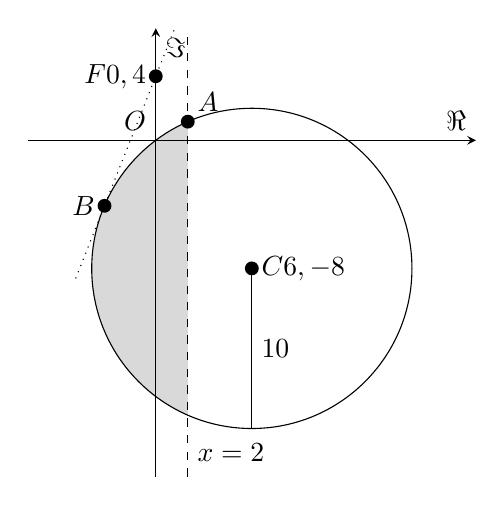
\begin{tikzpicture}[trim axis left, trim axis right]
                \begin{axis}[
                    samples = 101,
                    axis y line=middle,
                    axis x line=middle,
                    xtick = \empty,
                    ytick = \empty,
                    xmin=-8,
                    xmax=20,
                    ymin=-21,
                    ymax=7,
                    axis equal image,
                    axis on top,
                    xlabel = {$\Re$},
                    ylabel = {$\Im$},
                    legend cell align={left},
                    legend pos=outer north east,
                    after end axis/.code={
                        \path (axis cs:0,0) 
                            node [anchor=south east] {$O$};
                        }
                    ]

                    \coordinate[label=above right:$A$] (A) at (2, 1.165);
                    \coordinate[label=right:$C\bp{6,-8}$] (C) at (6, -8);
                    \coordinate[label=left:$F\bp{0, 4}$] (F) at (0, 4);
                    \coordinate[label=left:$B$] (B) at (-3.2, -4.09);
                    \coordinate (O) at (0, 0);

                    \begin{scope}
                        \clip (-8,-20) rectangle (2,7);
                        \fill[gray!30] (C) circle[radius=10];
                    \end{scope} 
            
                    \draw (C) -- (6,-18);
                    \node[anchor=west] at (6,-13) {10};
            
                    \draw (C) circle[radius=10];

                    \fill (A) circle[radius=2.5pt];
                    \fill (B) circle[radius=2.5pt];
                    \fill (C) circle[radius=2.5pt];
                    \fill (F) circle[radius=2.5pt];

                    \plot[dotted] {4 + 2.525*x};

                    \draw[dashed] (2, -21) -- (2, 7);
                    \node[anchor=west] at (2, -19.5) {$x = 2$};
                \end{axis}
            \end{tikzpicture}
        \end{center}
    \end{ppart}
    \begin{ppart}
        Let $A(x, y)$ be the point of intersection between the circle and the line $x = 2$, with $y > 0$. The equation of the circle is \[(x-6)^2 + (y+8)^2 = 10^2.\] Substituting $x = 2$ and solving gives $A(2, 2\sqrt{21} - 8)$. Thus, \[\sup \arg{z - 4\i} = \arg{\bs{2 + (2\sqrt{21} - 8)\i} - 4\i} = \arctan \frac{2\sqrt{21} -8 -4}{2} = -0.956 \tosf{3}.\]

        Set $F(0, 4)$. Let $B$ lie on the circumference of the circle such that $BF$ is tangent to the circle, with negative $y$-coordinate. Let $C(6, -8)$ be the centre of the circle. Note that \[FB = \sqrt{6^2 + (4+8)^2} = 6\sqrt{5}.\] Thus, \[\sin \angle CFB = \frac{CB}{BF} = \frac{10}{6\sqrt{5}} \implies \angle CFB = 0.84107 \tosf{5}.\] Next, we note that $C$ is at an angle \[\arg{6-8\i - 4\i} = \arctan \frac{-12}{6} = -1.10715 \tosf{5}\] relative to $F$. Thus, \[\min \arg{z-4\i} = -1.10715 - 0.84107 = -1.95 \tosf{3}.\]

        Hence, $-1.95 \leq \arg{z-4\i} < -0.856$.
    \end{ppart}
\end{solution}

\begin{problem}
    The tangent plant to the point $(a, b, c)$ on the surface with equation $(x-3)^2 + (y-5)^2 + z^2 = 4$ is a subspace of $\RR^3$. Find the range of values of $a$.
\end{problem}
\begin{solution}
    Note that the tangent plane must pass through the origin, since it is a subspace of $\RR^3$. Observe also that the equation $(x-3)^2 + (y-5)^2 + z^2 = 4$ describes a sphere with radius 2 and centre $(3, 5, 0)$. Since the sphere is symmetric about the $xy$-plane, the extremal points of $c$ occur on the $xy$-plane. Thus, it suffices to look at the projection of the sphere and the tangent plane on the $xy$-plane. There, the sphere becomes the circle with equation \[(x-3)^2 + (y-5)^2 = 4,\] while the tangent plane becomes the line $y = kx$ passing through the origin. Solving both simultaneously, we get the quadratic \[\bp{1 + k^2} x^2 - (6 + 10k)x + 30 = 0.\] Since $y = kx$ is tangent to the circle, the discriminant of this quadratic must be 0. Hence, \[(6 + 10k)^2 - 4\bp{1 + k^2}(30) = 0 \implies k = \frac{15 \pm 2\sqrt{30}}{5}.\] By the quadratic formula, the $x$-coordinates of the point of tangency are thus \[x = \frac{6+10k}{2\bp{1 + k^2}} = 1.04, \, 4.26.\] Hence, $1.04 \leq c \leq 4.26$, $c \neq 3$.
\end{solution}

\clearpage
\begin{problem}
    A spherical zone is the portion of the curved surface area of a sphere between two parallel planes $h$ units apart as shown in the diagram below.

    \begin{figure}[H]
        \centering
        \scalebox{0.6}{\import{media}{sphere.pdf_tex}}
    \end{figure}

    By using a suitable curve and rotation axis, explain if the location of the two planes will affect the curved surface area of the spherical zone.
\end{problem}
\begin{solution}
    Consider the rotation of the region bounded by $y = 0$, $x = a$, $x = b$ and $y = \sqrt{r^2 - x^2}$ about the $x$-axis, with $b-a = h$. The surface area of the resulting solid is precisely the curved surface area of a sphere of radius $r$.

    Note that \[1 + \bp{\der{y}{x}}^2 = 1 + \bp{\frac{-x}{\sqrt{r^2-x^2}}}^2 = 1 + \frac{x^2}{r^2 - x^2} = \frac{r^2}{r^2-x^2}.\] Thus, the surface area of revolution is \[2\pi \int_a^b \sqrt{r^2 - x^2} \sqrt{1 + \bp{\der{y}{x}}^2} \d x = 2\pi \int_a^b r \d x = 2\pi r (b-a) = 2\pi r h \units[2],\] which is independent of $a$ and $b$.
\end{solution}

\begin{problem}
    The region enclosed by the curve $y = x \ln x$, the $x$-axis and the vertical line $x = 2$ is rotated by $2\pi$ radians about the $y$-axis to form a solid.

    \begin{enumerate}
        \item Show that the volume of the solid is $\int_1^2 2\pi g(x) \d x$, where $g(x)$ is a function to be determined. Hence, find the exact volume of the solid.
        \item Using Simpson's Rule with $n = 4$ strips, estimate the value of the integral $\int_1^2 2\pi g(x) \d x$ up to 4 decimal places. You may assume that the intervals are equally spaces.
        \item Calculate the percentage error in your answer in part (b).
        \item Without performing the calculations to find an approximation using the Trapezium Rule, explain with reasoning whether your answer will be an over-estimate or under-estimate.
    \end{enumerate}
\end{problem}
\begin{solution}
    \begin{ppart}
        Note that $y$ intersects the $x$-axis when $x = 0$ or $x = 1$. By the shell method, the volume of revolution is \[V = 2\pi \int_1^2 xy \d x = 2\pi \int_1^2 x^2 \ln x \d x.\] Thus, $g(x) = x^2 \ln x$. Integrating by parts, we get
        \begin{align*}
            V &= 2\pi \bp{\evalint{\frac{x^3 \ln x}{3}}12 - \frac{1}{3} \int_1^2 x^2 \d x}\\
            &= 2\pi \evalint{\frac{x^3 \ln x}{3} - \frac{x^3}{9}}12\\
            &= \frac{2\pi}{9} \bp{24 \ln 2 - 7} \units[3].
        \end{align*}
    \end{ppart}
    \begin{ppart}
        Using Simpson's rule, we have the estimate \[\int_1^2 2\pi g(x) \d x \approx 2\pi \cdot \frac{0.5}{6} \bs{g(1) + 4g(1.25) + 2g(1.5) + 4g(1.75) + g(2)} = 6.7267 \todp{4}.\]
    \end{ppart}
    \begin{ppart}
        The percentage error in the estimate is \[\frac{\abs{6.7267 - \frac{2\pi}{9} \bp{24 \ln 2 - 7}}}{\frac{2\pi}{9} \bp{24 \ln 2 - 7}} = 0.00254\%.\]
    \end{ppart}
    \begin{ppart}
        Since $y = x^2 \ln x$ is concave upwards on $(1, 2)$, the trapezium rule will give an overestimate.
    \end{ppart}
\end{solution}

\begin{problem}
    A differential equation is given by \[\cos x \der{y}{x} - y \sin x = 2 \cos x,\] where $-\pi/2 < x < \pi/2$.

    \begin{enumerate}
        \item Show that the general solution of the differential equation is $y = 2 \tan x + C \sec x$, where $C$ is the arbitrary constant.
        \item Explain why the solution curves have turning points when $C < -k$ or when $C > k$, where $k$ is a constant to be determined.
        \item On the same diagram, sketch the family of solution curves where $C \neq -k$ or $k$.
    \end{enumerate}
\end{problem}
\begin{solution}
    \begin{ppart}
        We have \[\der{}{x} \bp{y \cos x} = 2\cos x.\] Integrating with respect to $x$, we get \[y \cos x = \int 2 \cos x \d x = 2\sin x + C.\] Thus, $y = 2 \tan x + C \sec x$.
    \end{ppart}
    \begin{ppart}
        Differentiating $y$, we get \[\der{y}{x} = 2\sec^2 x + C \sec x \tan x.\] For turning points, $\derx{y}{x} = 0$, thus \[2 + C \sin x = 0 \implies \sin x = -\frac{2}{C}.\] But $\sin x$ has range $[-1, 1]$, thus $C < -2$ or $C > 2$, i.e. $k = 2$.
    \end{ppart}
    \begin{ppart}
        \begin{figure}[H]\tikzsetnextfilename{527}
        \centering
        \begin{tikzpicture}[trim axis left, trim axis right]
            \begin{axis}[
                domain = -1.5:1.5,
                xmin = -1.7,
                xmax = 1.7,
                ymin = -8,
                ymax = 8,
                samples = 101,
                axis y line=middle,
                axis x line=middle,
                xtick = \empty,
                ytick = \empty,
                xlabel = {$x$},
                ylabel = {$y$},
                legend cell align={left},
                legend pos=outer north east,
                after end axis/.code={
                    \path (axis cs:0,0) 
                        node [anchor=north east] {$O$};
                    }
                ]
                \addplot[plotRed] {2*tan(\x r) - 3*sec(\x r)};
                \addlegendentry{$C < -2$};

                \addplot[black] {2*tan(\x r)};
                \addlegendentry{$-2 \leq C \leq 2$};

                \addplot[plotBlue] {2*tan(\x r) + 3*sec(\x r)};
                \addlegendentry{$C > 2$};
            \end{axis}
        \end{tikzpicture}
    \end{figure}
    \end{ppart}
\end{solution}

\begin{problem}
    \begin{enumerate}
        \item Let $z = \cos \t + \i \sin \t$. By considering $z^5$, show that \[\sin 5\t = 16\sin^5 \t - 20 \sin^3 \t + 5 \sin \t.\]
        \item Using your result in part (a),
        \begin{enumerate}
            \item find the distinct real roots to the equation \[16x^5 - 20x^3 +5x + 1 = 0,\] giving your answer, where appropriate, in exact trigonometric form; and
            \item find the exact value of $\tan[2]{\pi/5}$.
        \end{enumerate}
    \end{enumerate}
\end{problem}

\begin{problem}
    The polar curves $C_1$ and $C_2$ are given by the following equations in the respective intervals.

    \begin{alignat*}{2}
        C_1: r &= 2 + 2\sin \t, &\quad 0 \leq \t \leq 2\pi,\\
        C_2: r &= -2\sin\t, &\quad \pi < \t < 2\pi.
    \end{alignat*}

    \begin{enumerate}
        \item On a single diagram, sketch $C_1$ and $C_2$.
    \end{enumerate}

    The region $R$ is enclosed by the polar curves $C_1$ and $C_2$ in the third and fourth quadrants.

    \begin{enumerate}
        \setcounter{enumi}{1}
        \item Show that the perimeter of the region $R$ can be expressed as \[4 \int_p^q \sqrt{2 + 2 \sin \t} \d \t + \frac{2\pi}3,\] where $p$ and $q$ are exact real numbers to be determined. Evaluate this integral in exact form. You may use the identity \[1 + \sin \t = 2\sin[2]{\frac\t2 + \frac\pi4}\] without proof.
    \end{enumerate}
\end{problem}

\begin{problem}
    In a population of plants, a particular gene has two versions (called alleles): $A$ and $a$. A genotype is a combination of two alleles. Hence, for this particular gene, individual plants can have one of three genotypes: $AA$, $Aa$ or $aa$. The order of the sequence of genotypes does not matter.

    To breed a new plant, two plants, termed as its parents, are used. The new plane will inherit one gene from each of its parents' pairs of genes to form its own particular pair. For example, if one parent is of genotype $Aa$, it is equally likely that the new plant will inherit an $A$ gene or an $a$ gene from that parent, and if the other parent is of genotype $aa$, the new plant will definitely inherit an $a$ gene from that parent. Thus, the new plant will either be of genotype $Aa$ or $aa$.

    Suppose a farmer has a large population of plants consisting of some distribution of all three possible genotypes $AA$, $Aa$ and $aa$. He starts a breeding programme where each plant in the population is always bred with a plant with genotype $Aa$ to produce the next generation of plants.

    Let the vector $\cveciii{p_i}{q_i}{r_i}$ represent the proportion of plants with genotype $AA$, $Aa$ and $aa$ respectively in generation $i$, and $T : \RR^3 \to \RR^3$ be the transformation that maps $\cveciii{p_i}{q_i}{r_i}$ to $\cveciii{p_{i+1}}{q_{i+1}}{r_{i+1}}$.

    \begin{enumerate}
        \item Show that \[T: \cveciii{p_i}{q_i}{r_i} \mapsto \begin{pmatrix}2\b & \b & 0 \\ 2\b & 2\b & 2\b \\ 0 & \b & 2\b\end{pmatrix} \cveciii{p_i}{q_i}{r_i},\] where $\b$ is a non-zero constant to be determined. Find the nullity of $T$.
        \item Find the eigenvalues of $T$ and their corresponding eigenvectors of $T$.
        \item By diagonalizing the matrix representing $T$, find the proportion of the plants in the long run.
    \end{enumerate}
\end{problem}

\begin{problem}
    Two tanks are filled with salt water and are interconnected by pipes as shown below:

    \begin{figure}[H]
        \centering
        \import{media}{tank_prelim.pdf_tex}
    \end{figure}

    Tank $X$ and Tank $Y$ initially contain 600 litres and 500 litres of salt solution respectively.

    Salt water with a concentration of 1 gram per litre of salt enters Tank $X$ at a rate of 2 litres per minute. Pure water enters Tank $Y$ at a rate of 13 litres per minute. Through the connecting pipes, the salt solution in Tank $X$ flows into Tank $Y$ at 12 litres per minute. To keep the levels of the tanks the same, salt solution in Tank $Y$ flows into Tank $X$ at 10 litres per minute, and drains out at 15 litres per minute. The amount of salt in Tank $X$ and $Y$ are denoted as $x$ grams and $y$ grams respectively.

    \begin{enumerate}
        \item Show that \[\der{x}{t} = 2 - \frac1{50} x + \frac1{50} y \quad \tand \quad \der{y}{t} = \frac1{50} x - \frac1{20} y.\]
        \item Find a second order differential equation involving $y$.
        \item Find the general solution of the differential equation found in part (b).
        \item Find the ratio of the amount of salt in tank $X$ to the amount of salt in tank $Y$ in the long run.
    \end{enumerate}
\end{problem}